\documentclass[12pt]{report}
%\usepackage{fancybox}
\usepackage{geometry}
\usepackage{amsmath}
\usepackage{txfonts}
\usepackage{layout}
\usepackage{setspace}
%\usepackage{mathptmx}
\geometry{a4paper, left=22mm, right=22mm, top=25mm, bottom=25mm}
\usepackage{wrapfig}
\usepackage[dvipdfm]{graphicx,hyperref}
\usepackage{mediabb}
\setstretch{1.3}
\title{\Huge\bf{Role of Noncollective Excitations in Low-Energy Heavy-Ion Fusion Reaction
and Quasi-Elastic Scattering}}
\author{\\\\\\\\\\\\\\\\\\\\\\\\\\\\{\it\Large Department of Physics, Faculty of Science, Tohoku University}\\\\
\Huge Shusaku Yusa}
\date{March, 2013}
\begin{document}


\chapter{Introduction}
\setcounter{page}{1}
\pagenumbering{arabic}

Nuclear reactions show a variety of behaviors depending on the
colliding energy and species of the colliding nuclei. 
For heavy-ion reactions, a cancellation of
an attractive nuclear potential and the 
repulsive Coulomb
potential makes a potential barrier called the Coulomb barrier.
In Fig. \ref{potential}, we show an example of the potential
for $^{20}$Ne + $^{90}$Zr system.
In heavy-ion reactions around the Coulomb barrier energy, a quantum
tunneling effect is important for discussing the barrier penetration
and thus the fusion process.
Since a nucleus is a composite system, the internuclear potential can be
modified due to the internal excitations of the colliding nuclei,
and the fusion probability can be changed.
Therefore, heavy-ion reactions around the Coulomb barrier provide us with
a good opportunity to investigate an interplay between the reaction process
and internal excitations in the colliding nuclei.
These internal excitations can be considered as environmental degrees
of freedom for the relative motion of the reaction.
Thus, low-energy heavy-ion reaction gives 
an example of the quantum tunneling in the presence of
the external environment.
The effects of the external environment on a quantum tunneling process
were studied in detail by Caldeira and Leggett\cite{CL81,CL83}.
They considered a system coupled to a number of harmonic oscillators
which act as the environment, and discussed the effect of
the energy dissipation to the
environmental degrees of freedom on the quantum tunneling rate.
In low-energy heavy-ion reactions, 
a well known example of the coupling effect is the enhancement
of subbarrier fusion cross sections,
compared to a prediction of a simple potential model\cite{dasgupta,L95}.
\begin{figure}[t]
  \begin{center}
    \includegraphics[clip,keepaspectratio,width=100mm]{figure/chapter1/potential_20Ne_90Zr.eps}
    \caption{The internuclear potential between $^{20}$Ne and $^{90}$Zr nuclei.
    The green dotted line and the red dashed line show the Coulomb and the
    nuclear potentials, respectively. The solid blue line is the total (Coulomb +
    nuclear) potential. $R_{\rm B}$ and $V_{\rm B}$ are the position and the
    height of the Coulomb barrier, respectively.}
    \label{potential}
  \end{center}
\end{figure}

In order to take into account such a coupling effect in the description of
low-energy heavy-ion reactions, a coupled-channels method has been employed.
This method expresses the wave function as a superposition of various channel
wave functions, and is employed not only
in nuclear physics but also in quantum chemistry
to describe the multi-dimensional tunneling phenomena.
In the framework of the coupled-channels method, one can consider 
coupling to several kinds of intrinsic motions, such as 
low-lying collective excited states, transfer channels, noncollective
excited states, and giant resonances.
Among these excitation channels, conventionally,
a few low-lying collective excitations of the colliding nuclei,
such as a vibrational mode in spherical nuclei or rotational
excitations in deformed nuclei, have 
been taken into account.
Transfer channels have been also sometimes taken into account in analyses, 
often in a simple way.
Noncollective excitations
have not taken into account explicitly in usual calculations.
This is because, among the internal excited states,
collective states strongly couple to the relative motion and thus most
likely to be excited.
In fact, by taking into account the coupling to
low-lying collective states,
the large enhancement of subbarrier fusion cross sections observed in the
experiments has been accounted for various systems.
Although giant resonances have the collective nature,
these are not taken into account, either.
Their excitation energy is high enough,
and their effect can
be compensated by renormalizing the internuclear potential in the
coupled-channels calculations.
There are other reasons why only the low-lying 
collective excitations have been taken into account.
That is, the description of the collective states is relatively easy,
because their nature has been known much better than
noncollective states.
In addition, since a small number of the collective excitation channels,
at most a few tens of channels, are relevant to low-energy
heavy-ion reactions, it has been feasible to
take into account them explicitly in the actual calculations.
Including collective excitations,
the coupled-channels analyses have been successfully accounted for 
various experimental data for heavy-ion fusion reactions as well as quasi-elastic
scattering (a sum of elastic and inelastic scattering and transfer reactions)
at backward angles\cite{dasgupta}.
These two reaction processes are complementary to each other from the point of
view of the tunneling of the potential barrier. That is, 
the fusion process corresponds to the penetration of the barrier,
while the backward scattering corresponds to the reflection from the barrier.

In the eigenchannel representation, the channel-coupling effects lead to a
distribution of potential barriers\cite{DLW83}. It has been well established
that the barrier distribution can be directly extracted from experimental fusion
and quasi-elastic scattering cross sections.
For fusion reactions, the barrier distribution is defined as the second
derivative of the product of center-of-mass energy $E_{\rm c.m.}$ and the fusion
cross section $\sigma_{\rm fus}$ with respect to $E_{\rm c.m.}$, that is,
$d^2(E_{\rm c.m}\sigma_{\rm fus})/dE^2_{\rm c.m.}$\cite{L95,fusionbar}.
For quasi-elastic scattering, the barrier distribution is defined as the first
derivative of the ratio of the quasi-elastic scattering cross section to the Rutherford
cross section with respect to the center-of-mass energy at backward angle, that is,
$-d(\sigma_{\rm qel}(\theta=\pi)/\sigma_{\rm R}(\theta=\pi))/dE_{\rm c.m.}$
\cite{timmers, HR04}.
It has been well recognized that the fusion and
quasi-elastic barrier distributions behave in a similar way, while the
quasi-elastic barrier distribution tends to be more smeared\cite{timmers,HTK97,zamrun}.
These quantities are known to be considerably 
sensitive to the channel-coupling
effects\cite{dasgupta,L95,BT98}.
Since the barrier distribution represents the barriers which have to be
overcome by the colliding nuclei to fuse, 
it is a useful quantity for the understanding of the reaction process.
They can also serve for the determination of deformation parameters\cite{LRL93}.

Although the coupled-channels method has been successfully accounted for various
experimental data for heavy-ion fusion reactions, as well as quasi-elastic
scattering,
there also exist experimental data which cannot be accounted for by the conventional
coupled-channels analysis. One of the well known examples is a fusion experiment for
$^{40}$Ca + $^{90,96}$Zr systems\cite{TCS97}. 
In these systems, compared to the data for $^{40}$Ca
+ $^{90}$Zr system, subbarrier fusion cross sections for $^{40}$Ca + $^{96}$Zr
are strongly enhanced and the corresponding fusion barrier distribution
exhibits much smeared structure.
These behaviors have been attributed to the effect of
multi-nucleon transfer process, and cannot be accounted for by the
conventional calculations.
For the coupled-channels approach,
there is also a long-standing problem, that is, in order
to reproduce experimental fusion data, a significantly larger value of the
surface diffuseness of the nuclear potential is required, compared to the value
found from fitting to the scattering process\cite{MHD07,N04}.
Another long-standing problem is that
the coupled-channels calculation has not been able to
simultaneously reproduce the fusion and quasi-elastic barrier distributions for
$^{16}$O + $^{144}$Sm system\cite{zamrun}.

These failure and problems of the coupled-channels method indicate 
that the collective excitations are insufficient to understand the
reactions process for some systems, and other effects not included
in the conventional method, such as, noncollective excitations,
multi-nucleon transfer processes, or effects which are beyond
the framework of the ordinary coupled-channels method are also 
important to describe the reactions. 
For example, as we have mentioned, the multi-nucleon
transfer reactions have been
considered to be important for $^{40}$Ca + $^{96}$Zr system.
Nevertheless, these channels have not yet been taken
into account in the usual
calculations, since the description method of them 
has not been established.
Therefore, the study of multi-nucleon transfer reactions
as well as noncollective excitations
in heavy-ion reactions is important for the further understanding of reaction
process and for the development the coupled-channels method.
\begin{figure}[t]
  \begin{center}
    \begin{minipage}[t]{73mm} 
    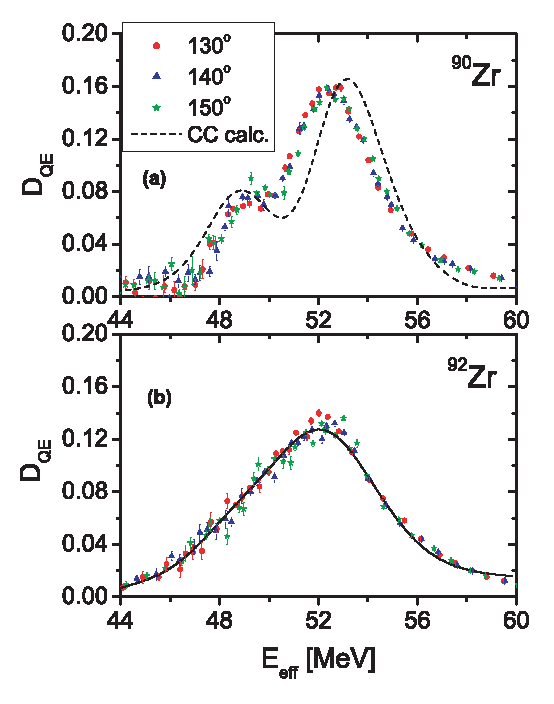
\includegraphics[clip,keepaspectratio,width=73mm]{figure/chapter1/qel_bar_dist_20Ne_9092Zr.eps}
      \caption{Extracted quasi-elastic barrier distribution for $^{20}$Ne +
               $^{90,92}$Zr systems at three scattering angles. The dashed
               line in Fig. \ref{fig1.2}(a) shows the result of the
               coupled-channels calculation. 
               The solid line in Fig. \ref{fig1.2}(b)
               is obtained by smearing the data for $^{20}$Ne
               + $^{90}$Zr system. The figure is taken from Ref.\cite{piasecki}.}
      \label{fig1.2}
    \end{minipage}
    \hspace{1.0cm}
    \begin{minipage}[t]{75mm}
      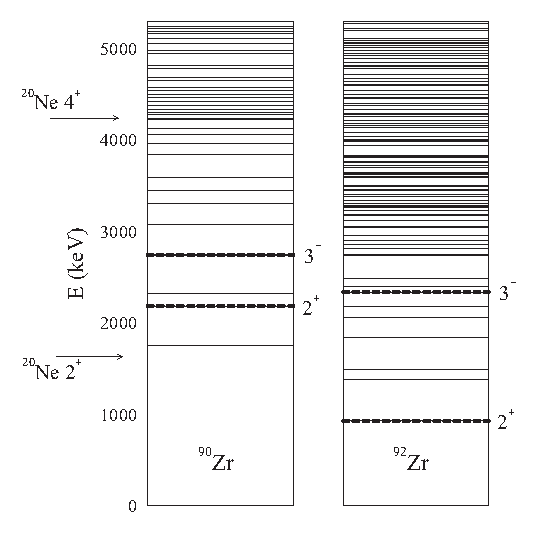
\includegraphics[clip,keepaspectratio,width=75mm]{figure/chapter1/Zr_spectra.eps}
      \caption{Energy spectra for Zr isotopes. The dashed lines represent the
      collective excitations which are
      taken into account in the coupled-channels 
      calculation shown in Fig. \ref{fig1.2}.
      The rotational states of $^{20}$Ne are also shown.
      Taken from Ref. \cite{piasecki}.}
      \label{fig1.3}
    \end{minipage}
  \end{center}
\end{figure}

\begin{figure}[t]
\center
    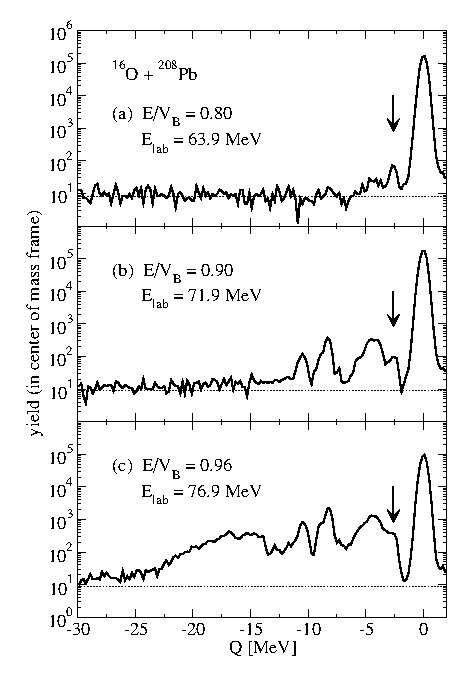
\includegraphics[clip,keepaspectratio,width=90mm]{figure/chapter1/Qdist_16O_208Pb.eps}
    \caption{Experimental Q-value distribution for $^{16}$O + $^{208}$Pb system
    at three subbarrier energies. The figure is taken from Ref. \cite{evers}.
    The peak indicated by the arrow represents the octupole phonon excitation of
    $^{208}$Pb.}
    \label{fig1.4}
\end{figure}

In addition to the long-standing problems which we have mentioned above,
several recently obtained data cannot be accounted for by the
conventional coupled-channels calculations.
For example, fusion cross sections at
deep subbarrier energies are strongly suppressed, compared to the prediction of
the coupled-channels calculations\cite{J02,JRJ04,DHD07,S08}.
Another example is the quasi-elastic scattering experiment for $^{20}$Ne +
$^{90,92}$Zr systems\cite{piasecki}.
In this experiment,
the quasi-elastic barrier distributions
were obtained from measured quasi-elastic cross sections 
and were analyzed by the
coupled-channels calculation.
This is shown in Fig. \ref{fig1.2}, which is taken from Ref. \cite{piasecki}.
The dots represent the experimental data at three different scattering angles and
the dashed line in the upper figure represents the results of
the coupled-channels calculation.
The difference in the scattering angles of the data is compensated
by modifying the CM energy $E_{\rm c.m.}$ 
to $E_{\rm eff}$, which takes into account the 
effect of the centrifugal potential (see Eq. (\ref{effective_E})).
As one can see, 
the experimentally obtained barrier distribution
behaves in a significantly
different way between the two systems, that is, the barrier distribution for
$^{20}$Ne + $^{92}$Zr is much more smeared than that for $^{20}$Ne + $^{90}$Zr
system. However, the coupled-channels calculation which takes into account the
rotational excitations of $^{20}$Ne and
the collective vibrational excitations of $^{90,92}$Zr
yields similar barrier distributions, because the largely deformed $^{20}$Ne
dominantly determines the barrier structure,
while the difference in the vibrational
excitations in $^{90,92}$Zr plays only a minor role.
One of the possible reasons for this problem is the effect of the transfer
reactions\cite{TCS97,T98}. However, for these systems,
the total transfer cross sections have been
found to be almost the same\cite{piasecki}. Therefore, the difference in the barrier
distributions has been conjectured to arise from noncollective excitations which
are not explicitly taken into account in the coupled-channels analysis.
In Fig. \ref{fig1.3}, we show the energy spectra of $^{90,92}$Zr nuclei.
Since the $^{90}$Zr is a closed shell nucleus with 50 neutrons and $^{92}$Zr has
two additional neutrons,
the number of relatively low-lying noncollective states
in $^{92}$Zr is much larger than that in $^{90}$Zr.
In fact, while there are only 12 states in the $^{90}$Zr nucleus up to 4 MeV,
there are 53 known states in $^{92}$Zr nucleus\cite{bnl}. For 5 MeV, the number
of known states is 35 and 87 for $^{90}$Zr and $^{92}$Zr, respectively.
Although the excitation to each noncollective state is weak compared to that to a collective
state, excitations to a large number of noncollective states may alter the barrier structure.


Indication of the importance of the noncollective excitations can be seen in
the quasi-scattering experiments 
for $^{16}$O + $^{208}$Pb system\cite{T96,T97,evers,lin,evers2}.
In the experiments, the Q-value distribution was measured at
several different energies.
The experimental data are shown in Fig. \ref{fig1.4}, which is taken from Ref.
\cite{evers}. $V_{\rm B}$ in the figure 
represents the height of the Coulomb barrier.
The horizontal axis represents the Q-value, that is, the loss of kinetic energy
due to the internal excitations of the colliding nuclei.
Thus, the peak at $Q = 0$ represents the elastic scattering and
the contribution from a negative Q-value represents the inelastic scattering.
The arrow in the figure indicates the peak for 
the first $3^-$ state in $^{208}$Pb
which is considered to be a collective state.
The distribution at larger Q-value can be considered as the contribution from the
noncollective excited states, since in such a high excitation energy region, a
large number of noncollective excited states exist in the energy spectrum
of $^{208}$Pb.
While the elastic scattering is
dominant at the lowest incident energy, the experimental data indicate that 
the contribution from the noncollective excitations
increases as the incident energy increases.
For this system,
precise fusion cross sections were measured around the Coulomb barrier
energy, and a careful coupled-channels analysis
has been performed\cite{MBD99,EM07} by including the collective vibrational
excitations in $^{208}$Pb and a few transfer channels.
Since both $^{16}$O and $^{208}$Pb are double closed shell nuclei,
one may think
that it is a straightforward task to reproduce the experimental data.
However, the coupled-channels calculation
cannot simultaneously reproduce the fusion cross sections above and below the
Coulomb barrier and
overestimates
the height of the main peak of the fusion barrier distribution, even if all the
relevant collective excitations are taken into account.
This fact shows that one has to take into account the effects which are
not taken into
account in the conventional coupled-channels calculation, such as noncollective
excitations.
Therefore, the experimental data for $^{16}$O + $^{208}$Pb system,
together with that for $^{20}$Ne + $^{90,92}$Zr system,
provide us with a good opportunity to
investigate the effect of noncollective excitations in heavy-ion reactions.

The aim of this thesis is thus to investigate the role of noncollective
excitations in low-energy heavy-ion fusion reactions and quasi-elastic
scattering. In the conventional coupled-channels calculations, the effect of
noncollective excitations is implicitly taken into account through the
optical potential. However, the distribution of eigenbarriers is not altered in
this treatment. Thus, by including the noncollective excitations into the
coupled-channels method in an explicit way, we discuss the role of
noncollective excitations in fusion and quasi-elastic scattering
cross sections and barrier distributions, as well as Q-value distributions.
This study will give us a further understanding of the reaction process,
which has usually been discussed only with the collective excitations.
It will be also an important step to develop the modern coupled-channels 
method and to extend the applicability of the method.

The thesis is organized as follows. 
In chapter 2, a fundamental feature of nuclear excited states is reviewed.
Especially, low-lying collective excited states are reviewed in detail based on
the liquid drop model. 
We also mention
an interpretation of the collective and the
noncollective excited states from a microscopic point of view.

In chapter 3, the theoretical framework for the description of heavy-ion reaction
is reviewed. The coupled-channels method is employed throughout this work.
After the derivation of the coupled-channels equations in the
full angular coupling formalism,
the isocentrifugal approximation is introduced to reduce the number of channels
in the calculation\cite{LR84,NRL86,NBT86,ELP87,T87,TMBR91,TAB92,AA94,GAN94,HTBB95}.
A sudden tunneling limit is discussed and the eigenchannel formalism is
presented.
The barrier distribution method is then introduced both for fusion reaction and
quasi-elastic scattering.
The constant coupling approximation is also discussed\cite{DLW83}.
The effect of collective excitations on subbarrier fusion cross
sections and the barrier distribution is
presented through typical calculations for the vibrational coupling and
the rotational coupling.
The effect of high-lying collective states is also discussed.
Inclusion of
high-lying states does not significantly
alter the shape of the barrier distribution
but produces an adiabatic potential
renormalization\cite{THAB94}.
At the end of chapter 3, the computational method of the coupling matrix
elements in the full order coupling is presented\cite{ccfull}.

In order to take into account the coupling to noncollective states in the
coupled-channels calculation, one needs to know the transition strength to those
states. For some nuclei, such information is experimentally obtained. For
example, almost all of the excited states of $^{208}$Pb up to 7 MeV have been
identified (the spin, parity, excitation energy, and deformation parameter)
from high precision proton inelastic scattering experiments\cite{WCHM75,LBF73}. 
However, in general, such information is not necessarily available.
For such systems, one has to resort to a theoretical or phenomenological
model to estimate the transition strength to the noncollective states.
For this purpose, 
a model for heavy-ion reactions based on the random matrix theory
is employed in this work.
This model was originally introduced for the study of heavy-ion deep inelastic
collisions in the 1970's by Weidenm\"uller and his
collaborators\cite{KPW76,AKW78,BSW78,akw1,akw2,akw3,akw4}.
Chapter 4 is devoted to the random matrix theory, which is the basis of this model.
Fundamental feature of this theory and the relation to the nuclear spectrum is
reviewed.

As mentioned above, the information on the noncollective excited states is obtained
for $^{208}$Pb nucleus from high precision proton inelastic scattering
experiments. Using this information, in chapter 5, we investigate the role of
the noncollective excitations of $^{208}$Pb in the reaction of $^{16}$O + $^{208}$Pb
system\cite{YHR12}.
Since the coupled-channels calculation has not successfully reproduced
the fusion cross sections and the fusion barrier distribution
for this system\cite{MBD99},
we shall study whether the noncollective excitations can improve the agreement
of the coupled-channels calculation with the experimental data.
Together with the noncollective excitations, the effect of anharmonicity is also
investigated, as the first excited state of $^{208}$Pb, which is the 
octupole phonon state at
2.615 MeV, has been found to have a finite quadrupole moment\cite{JBF77,BH83,FT90}.
The energy dependence of the Q-value distribution is also
investigated including the
noncollective excitations. Although the agreement of the calculation with the
experimental data is not improved for the fusion reaction,
the effect of the noncollective excitations has been found to small.
On the other hand, the energy dependence of the calculated 
Q-value distribution agrees with that of
the experimental Q-value distribution in a qualitative way.
At the end of this chapter, we investigate the
dependence of the effect of the noncollective excitations
on the mass number of the projectile nucleus.
We present the fusion calculations for $^{32}$S + $^{208}$Pb and
$^{40}$Ca + $^{208}$Pb systems and
show that the noncollective effect increases as the mass number of the projectile
increases.

In chapter 6, we investigate the role of noncollective excitations in
$^{20}$Ne + $^{90,92}$Zr systems.
For $^{90,92}$Zr nuclei, the information on the noncollective excited states is not
sufficiently obtained in contrast to $^{208}$Pb nucleus. 
Thus, one cannot use the same approach as in the calculation for
$^{16}$O + $^{208}$Pb reaction to describe the coupling to
the noncollective excited states.
Therefore, we employ the random matrix model for the description of the
noncollective excitations.
To see the applicability of the random matrix model, we first apply the model
to $^{16}$O + $^{208}$Pb reaction, and compare with the more reliable calculation 
which uses the experimentally obtained information on the noncollective states
of $^{208}$Pb.
The obtained results show that the random matrix model can reproduce the results
based on the experimental information.
We then apply the model to the $^{20}$Ne + $^{90,92}$Zr systems.
Using the same parameters in the random matrix model between the two systems,
we show that the noncollective
excitations smear the peak structure of the quasi-elastic barrier distribution
for $^{20}$Ne + $^{92}$Zr system,
while for $^{20}$Ne + $^{90}$Zr system, the
noncollective excitations do not
change the structure of the barrier distribution in a significant way.
Although the perfect agreement of the quasi-elastic scattering cross sections
with the data is not obtained by the noncollective excitations, we
show the magnitude of the noncollective effect is largely different
between $^{20}$Ne + $^{90,92}$Zr systems, and this
difference originates from the difference in the spectra of $^{90,92}$Zr nuclei.
We also apply the random matrix model to other systems which use $^{90}$Zr or
$^{92}$Zr as a target, and verify that the inclusion of the noncollective
excitations of $^{90,92}$Zr does not lead to an inconsistency with the experimental
data for these systems.
At the end of this chapter,
we apply the model to $^{24}$Mg + $^{90,92}$Zr systems. Since the $^{24}$Mg
is a prolately deformed nucleus with a large deformation parameter, one can expect
that the barrier distribution for the $^{24}$Mg + $^{90,92}$Zr systems exhibits a
behavior similar to the $^{20}$Ne + $^{90,92}$Zr systems.
Our results show that this is the case.

Finally the summary of the thesis is given in chapter 7.

\end{document}

